% !TeX root = ..\main.tex
\section{Thiết kế quy trình nghiệp vụ}

Các lược đồ BPMN được nhóm thiết kế trên app Bizagi.

\subsection{Quản lý kho}
\begin{figure}[!htp]
	\centering
	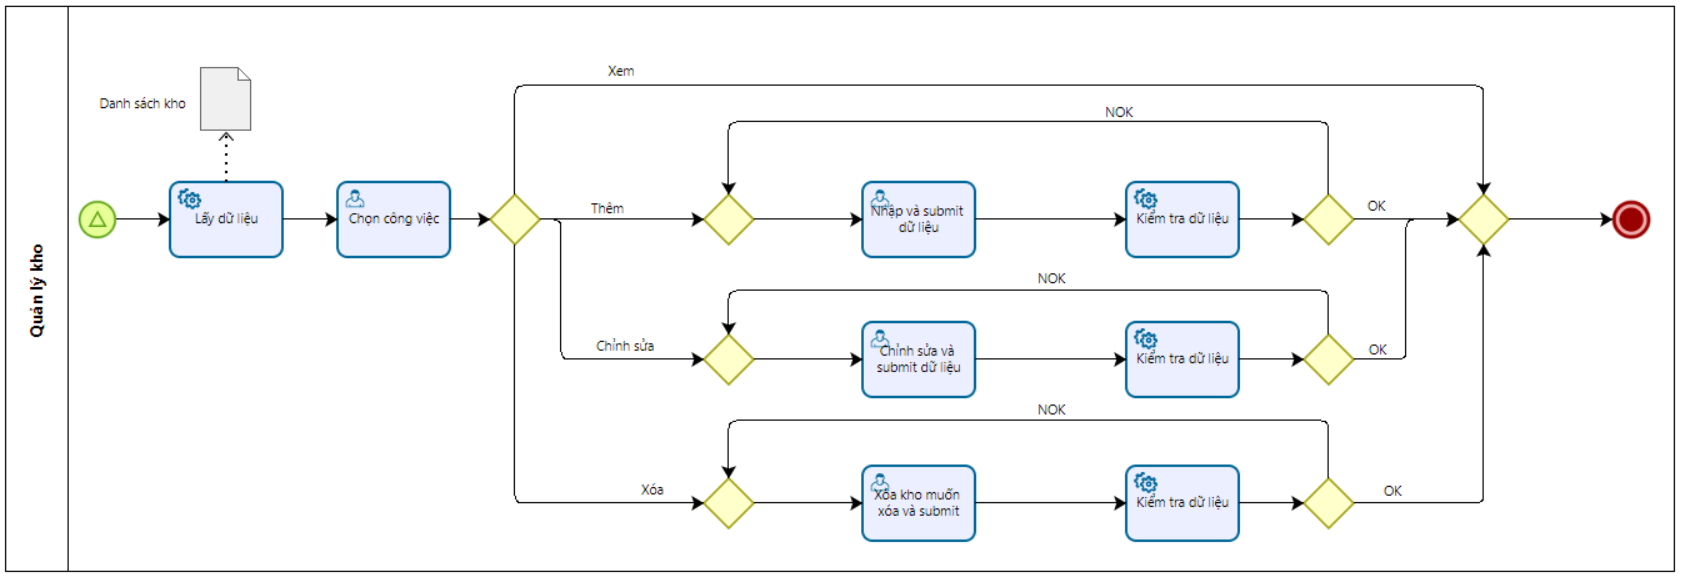
\includegraphics[width=17cm]{img/BPMN/Tho/warehouse.PNG}
	\newline
	\caption{Lược đồ BPMN cho quy trình quản lý kho}
\end{figure}

Quy trình bắt đầu khi người dùng truy cập vào giao diện quản lý kho. Hệ thống quản lý kho lấy ra dữ liệu kho cho người dùng thực hiện các tác vụ của mình. Nếu người dùng chỉ xem dữ liệu thì sẽ không có gì xảy ra thêm. Nếu người dùng thêm dữ liệu, người dùng sẽ nhập và submit dữ liệu mới, hệ thống kiểm tra và hoàn thành việc thêm nếu dữ liệu hợp lệ. Nếu người dùng chỉnh sửa dữ liệu, người dùng chỉnh sửa trên dữ liệu hiện tại của kho, hệ thống kiểm tra và hoàn thành việc cập nhật nếu dữ liệu hợp lệ. Nếu người dùng xóa dữ liệu, người dùng xóa kho và submit, hệ thống kiểm tra dữ liệu và hoàn thành việc xóa nếu dữ liệu hợp lệ.

\subsection{Khách hàng mua hàng}
\begin{figure}[!htp]
	\centering
	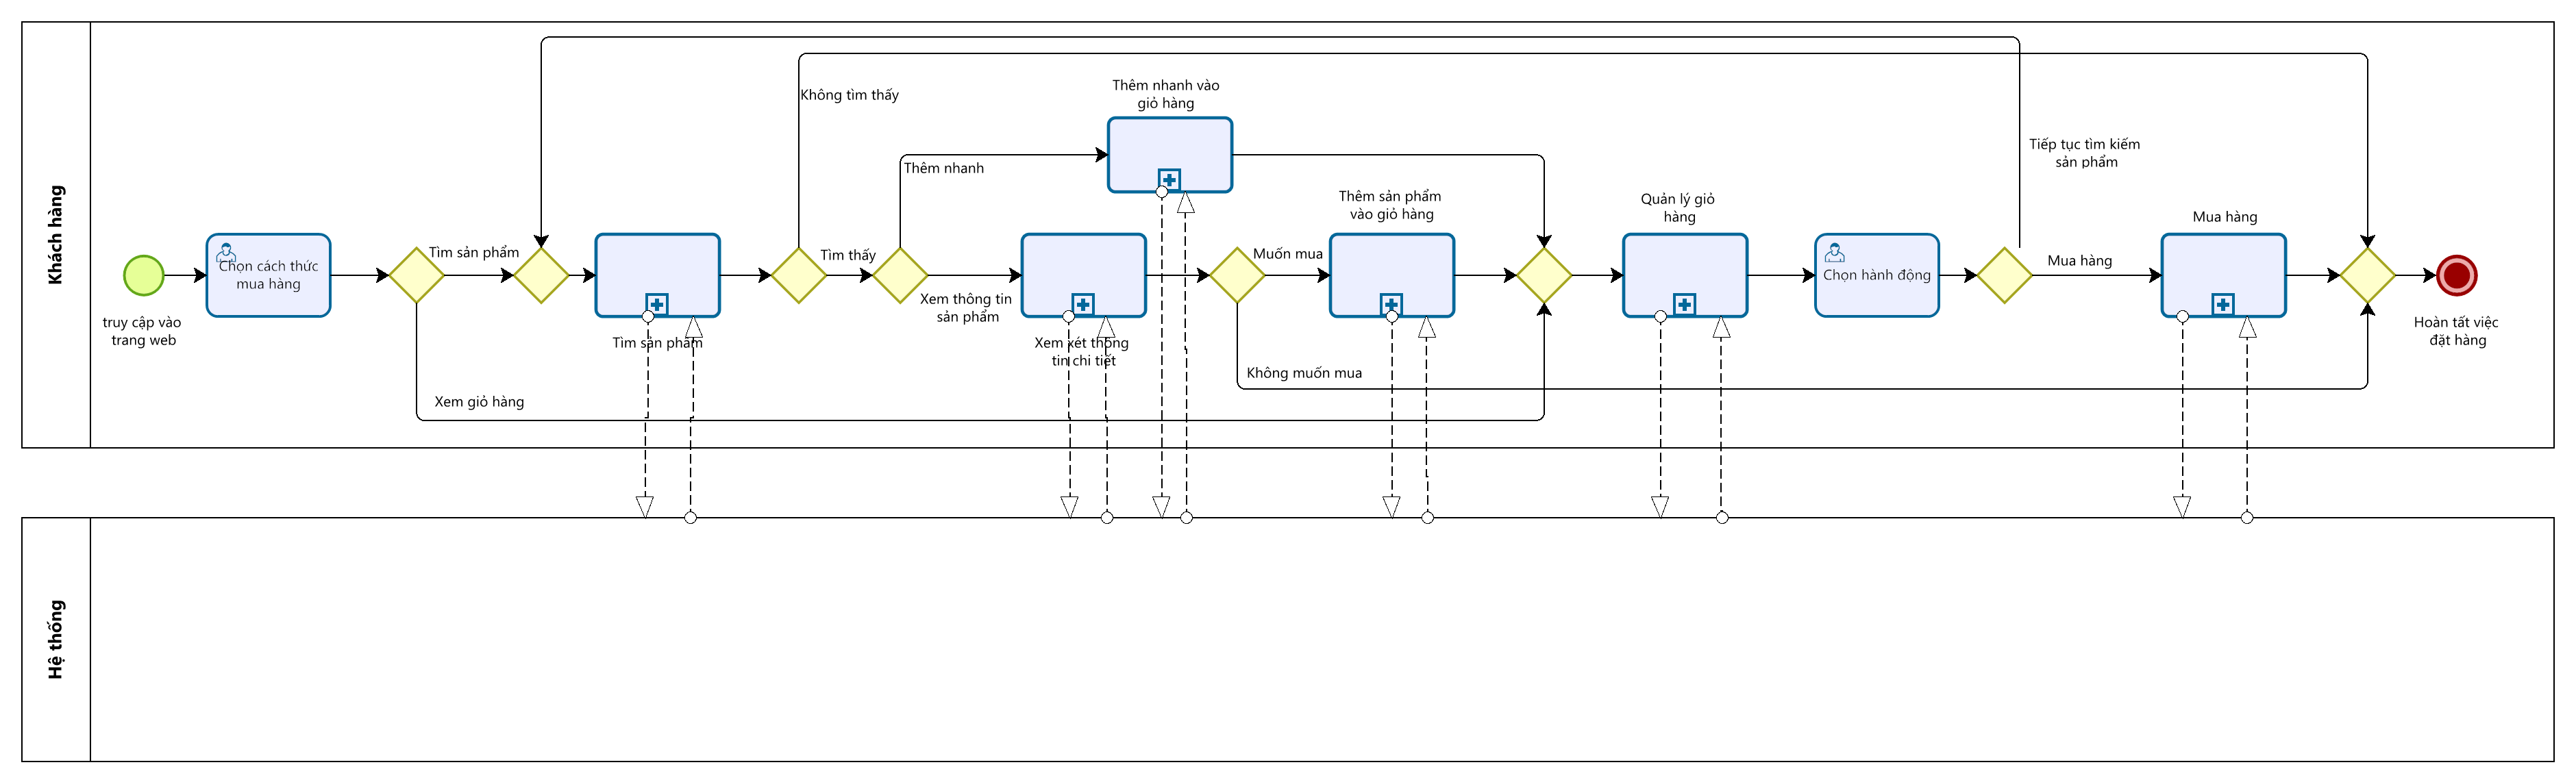
\includegraphics[width=17cm]{img/BPMN/customer_buy/customer_buy.png}
	\newline
	\caption{Lược đồ BPMN cho quy trình khách hàng mua hàng}
\end{figure}

Quy trình bắt đầu khi người dùng bắt đầu truy cập vào trang web, khách hàng chọn cách thức mua hàng là bắt đầu từ tìm sản phẩm hoặc là bắt đầu mua từ những sản phẩm đã có sẵn trong giỏ hàng. Khi người dùng chọn tìm sản phẩm thì người dùng sẽ thực hiện quy trình con "Tìm sản phẩm". Sau khi thực hiện xong tìm sản phẩm và tìm thấy thì người dùng thực hiện quy trình "xem thông tin chi tiết" để hiểu rõ hơn về sản phẩm và quyết định có muốn thêm sản phẩm vào giỏ hàng hay không. Sau khi thêm sản phẩm vào giỏ hàng thì người dùng thực hiện quy trình con quản lý giỏ hàng để lựa chọn cũng như cập nhật các đặc điểm mà người dùng mong muốn ở sản phẩm. Sau khi quản lý xong giỏ hàng thì người dùng cần chọn hành động tiếp tục tìm kiếm thêm sản phẩm để mua hàng hoặc là trực tiếp đi đến quy trình con "Mua hàng" và sau đó là kết thúc quy trình.


\begin{figure}[!htp]
	\centering
	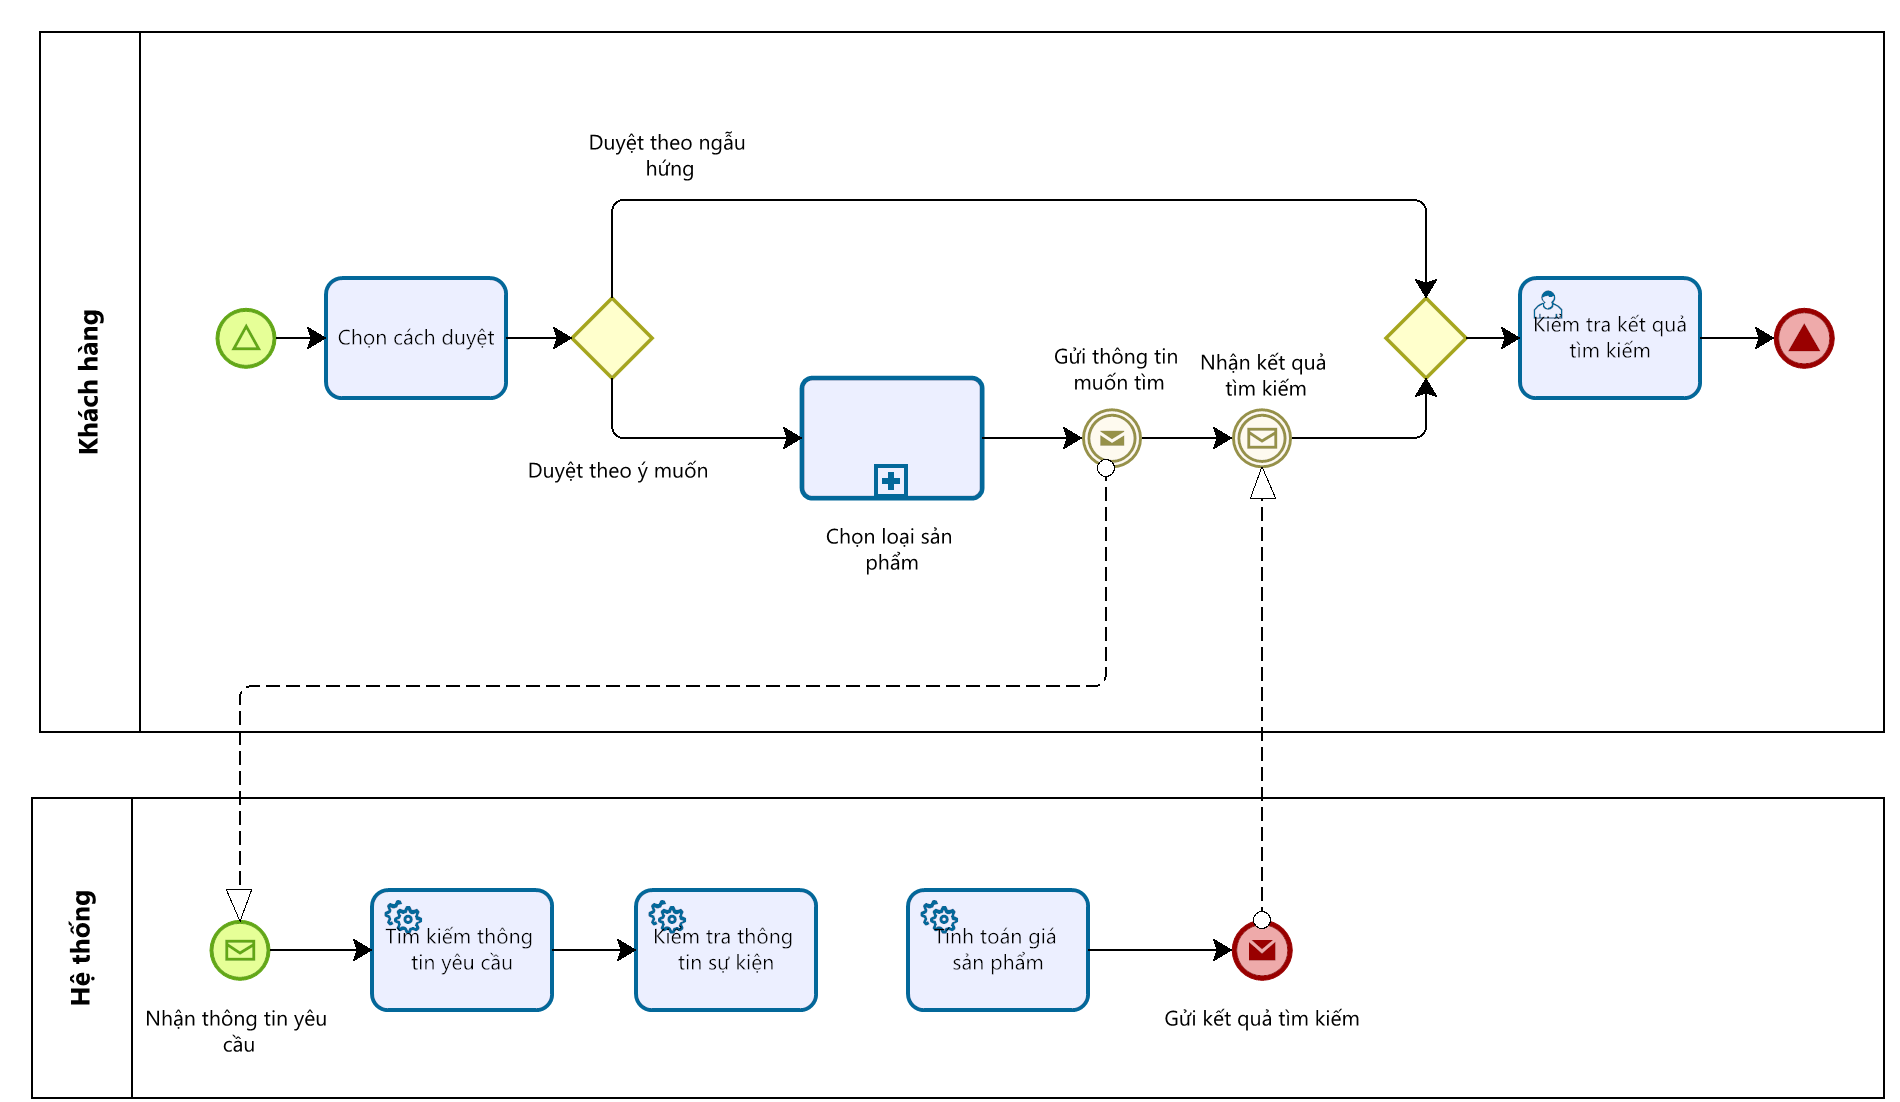
\includegraphics[width=11cm]{img/BPMN/customer_buy/customer_search_product.png}
	\newline
	\caption{Lược đồ BPMN cho quy trình con tìm kiếm sản phẩm}
\end{figure}

Đây là một quy trình con chứa quy trình tìm kiếm sản phẩm mà người dùng muốn tìm kiếm. Bắt đầu từ việc chọn cách duyệt bằng cách duyệt theo ngẫu hứng hay duyệt theo ý muốn. Khi người dũng duyệt theo ý muốn thì thực hiện quy trình con "Chọn loại sản phẩm" để chọn những loại sản phẩm theo ý muốn của khách hàng. Sau khi chọn loại sản phẩm thì hệ thống sẽ nhận thông tin và xử lý, sau đó phản hồi kết quả và người dùng kiểm tra kết quả tìm kiếm và kết thúc quy trình con này.

\begin{figure}[!htp]
	\centering
	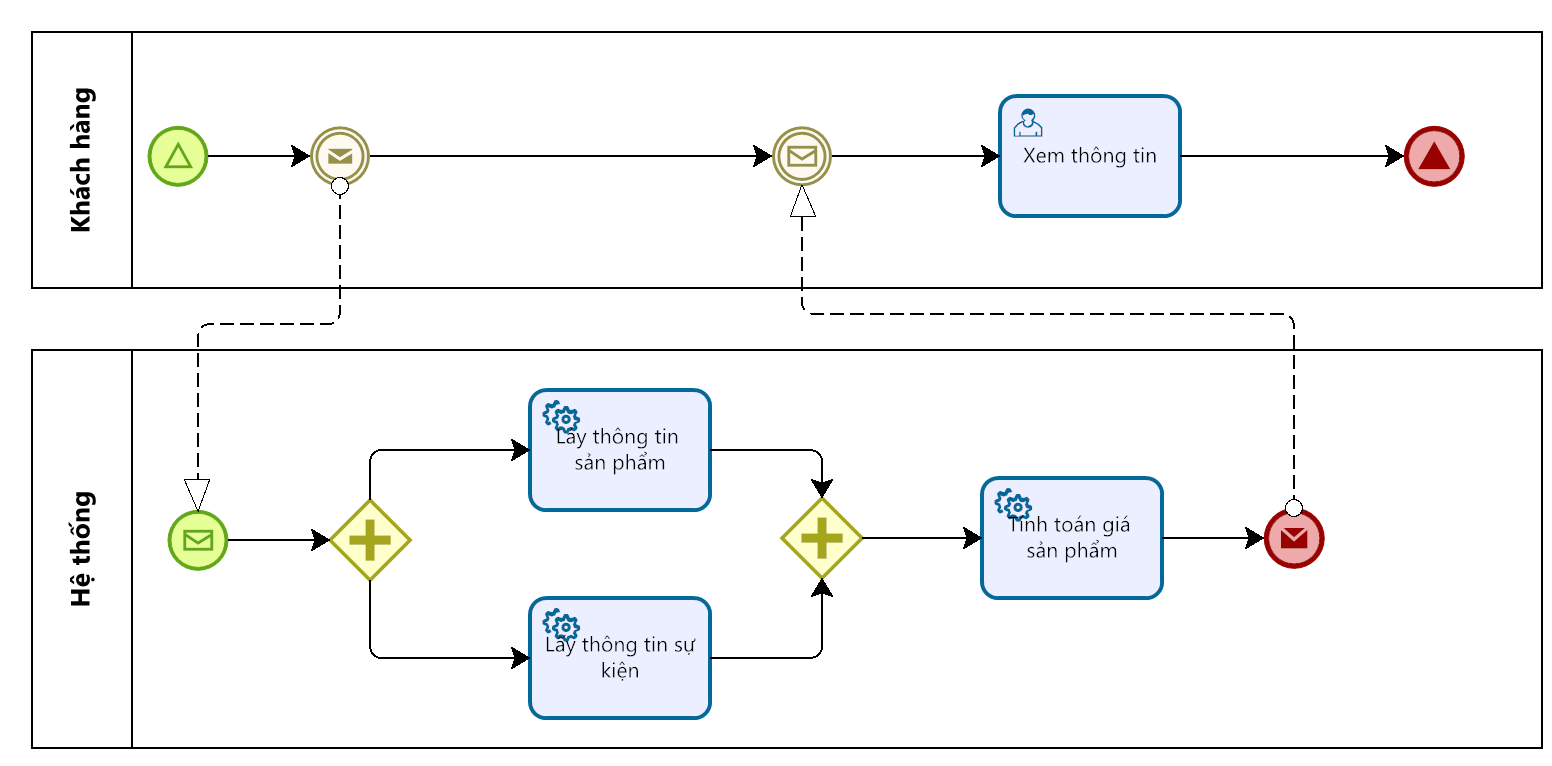
\includegraphics[width=9cm]{img/BPMN/customer_buy/customer_buy_product_detail.png}
	\newline
	\caption{Lược đồ BPMN cho quy trình con xem chi tiết sản phẩm}
\end{figure}

Đây là một quy trình con chứa quy trình xem chi tiết sản phẩm mà người dùng muốn tìm kiếm. Bắt đầu từ việc người dùng gửi thông tin cho hàng muốn tìm cho hệ thống. Hệ thống thực hiện tìm kiếm và tính toán, sau đó gửi thông tin cho khách hàng. Sau khi nhận được kết quả thì khách hàng xem thông tin chi tiết của sản phẩm và kết thúc quy trình.


\newpage
\begin{figure}[!htp]
	\centering
	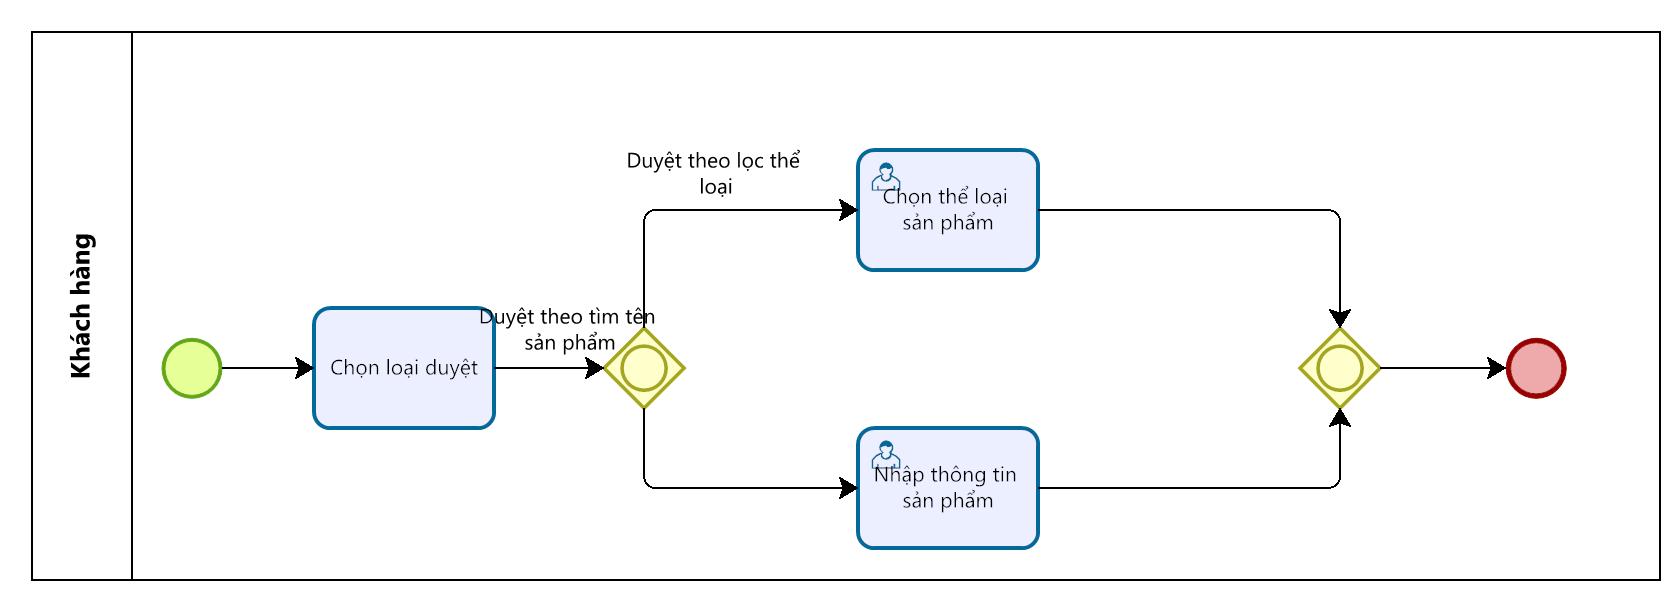
\includegraphics[width=9cm]{img/BPMN/customer_buy/customer_select_type.png}
	\newline
	\caption{Lược đồ BPMN cho quy trình con chọn loại sản phẩm mà khách hàng muốn tìm}
\end{figure}

Đây là một quy trình con chứa quy trình chọn loại sản phẩm mà người dùng muốn tìm kiếm. Bắt đầu từ việc chọn loại duyệt thì người dùng có thể chọn duyệt theo thể loại hoặc duyệt theo tên tìm kiếm.

\begin{figure}[!htp]
	\centering
	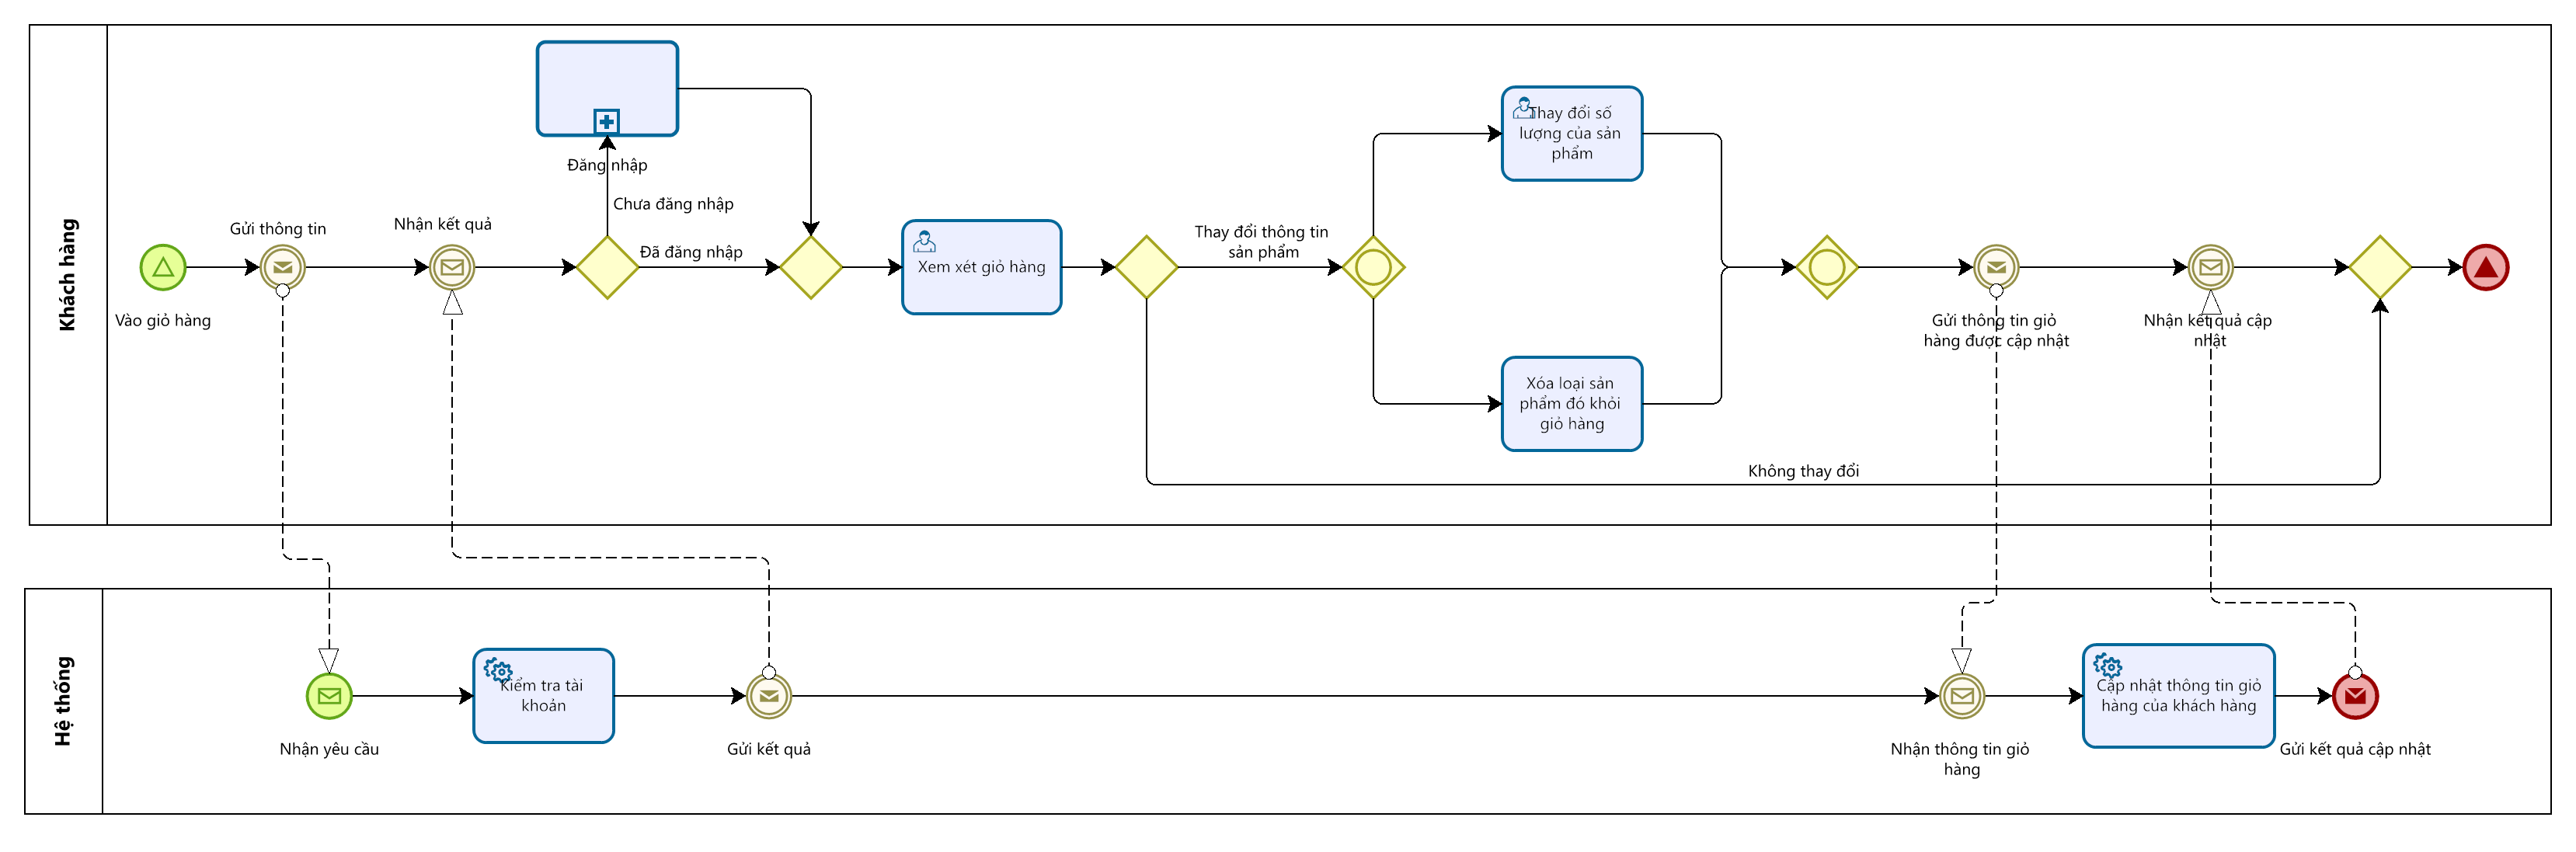
\includegraphics[width=14cm]{img/BPMN/customer_buy/customer_cart.png}
	\newline
	\caption{Lược đồ BPMN cho quy trình quản lý giỏ hàng}
\end{figure}

Đây là một quy trình con chứa quy trình quản lý giỏ hàng. Quy trình bắt đầu từ khi khách hàng chọn vào giỏ hàng. Hệ thống thực hiện kiểm tra tài khoản rồi sau đó truy xuất dữ liệu giỏ hàng của tài khoản khách hàng và phản hồi về lại cho khách hàng. Khách hàng thực thực hiện xem xét giỏ hàng và thực hiện thay đổi thông tin sản phẩm trong giỏ hàng bằng cách thay đổi thông tin sản phẩm hay xóa sản phẩm khỏi giỏ hàng, hệ thống nhận thông tin thay đổi sau đó kiểm tra thông tin và cập nhật thông tin giỏ hàng rồi trả về kết quả, khách hàng nhận kết quả và kết thúc quy trình.


\begin{figure}[!htp]
	\centering
	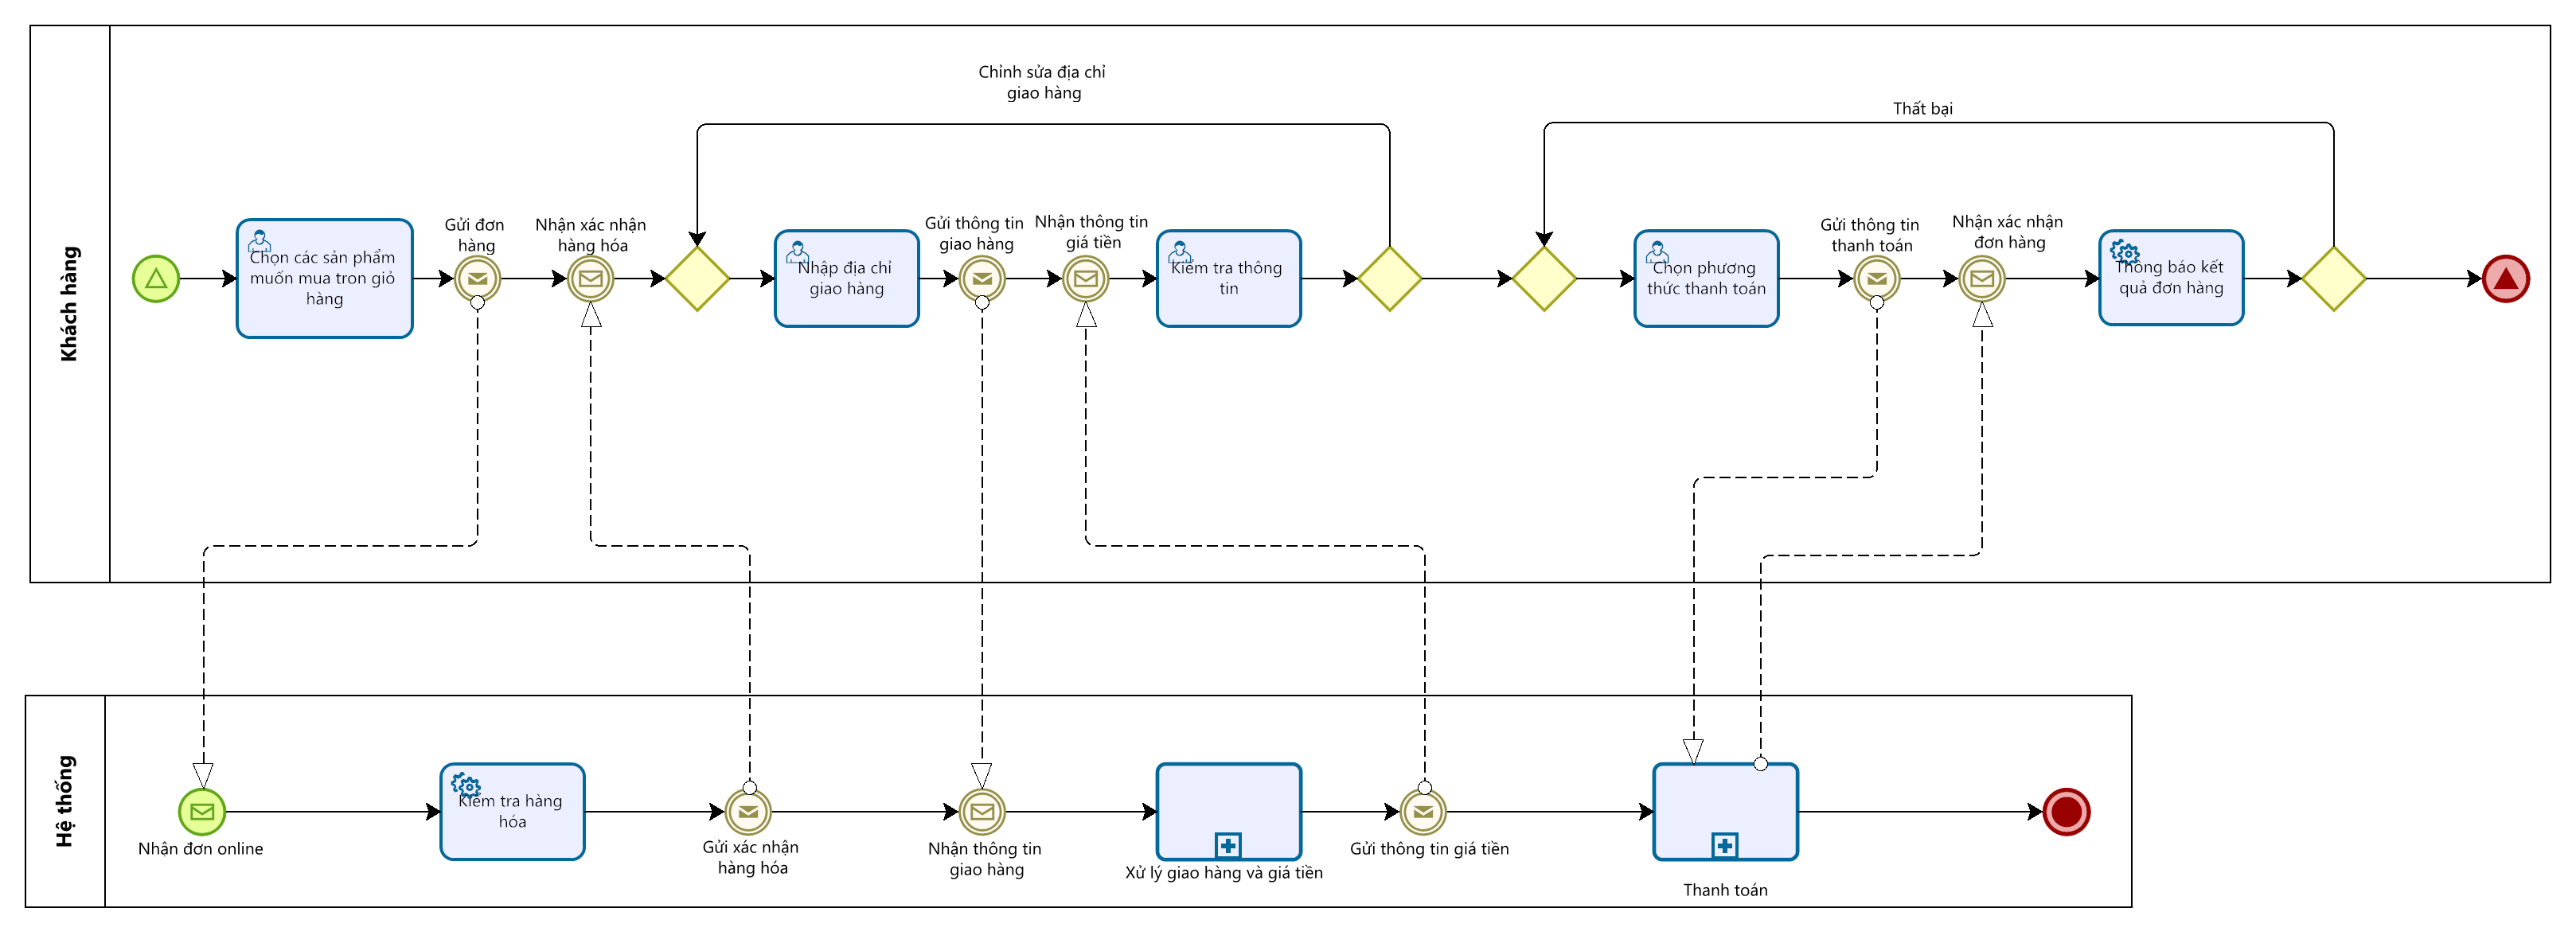
\includegraphics[width=17cm]{img/BPMN/customer_buy/customer_buy_order.png}
	\newline
	\caption{Lược đồ BPMN cho quy trình mua hàng}
\end{figure}

Đây là một quy trình con chứa quy trình đặt mua hàng của khách hàng. Khách hàng chọn các sản phẩm trong giỏ hàng mà bản thân muốn mua và chọn "Đặt hàng" và nhập địa chỉ giao hàng, hệ thống sẽ thực hiện tính toán giao hàng để tính tổng hóa hơn cho khách hàng. Khách hàng thực hiện kiểm tra thông tin sau khi nhận lại thông tin giá tiền, tiếp theo thực hiện chọn phương thức thanh toán và chọn "Thanh toán", khách hàng sẽ thực hiện thanh toán với bên thứ 3. Khi thanh toán thành công, hệ thống thực hiện tạo đơn hàng và phản hồi thông báo kết quả đơn hàng.

\begin{figure}[!htp]
	\centering
	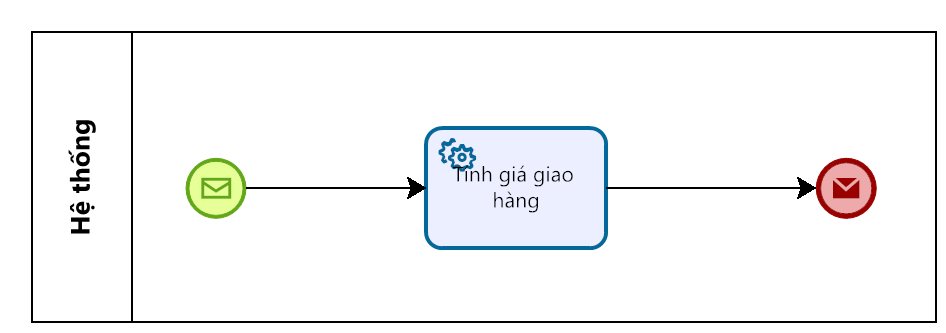
\includegraphics[width=5cm]{img/BPMN/customer_buy/customer_calc_fee.png}
	\newline
	\caption{Lược đồ BPMN cho quy trình tính toán chi phí giao hàng}
\end{figure}

Đây là một quy trình con thực hiện tính toán giá giao hàng giựa trên địa chi của khách hàng.

\begin{figure}[!htp]
	\centering
	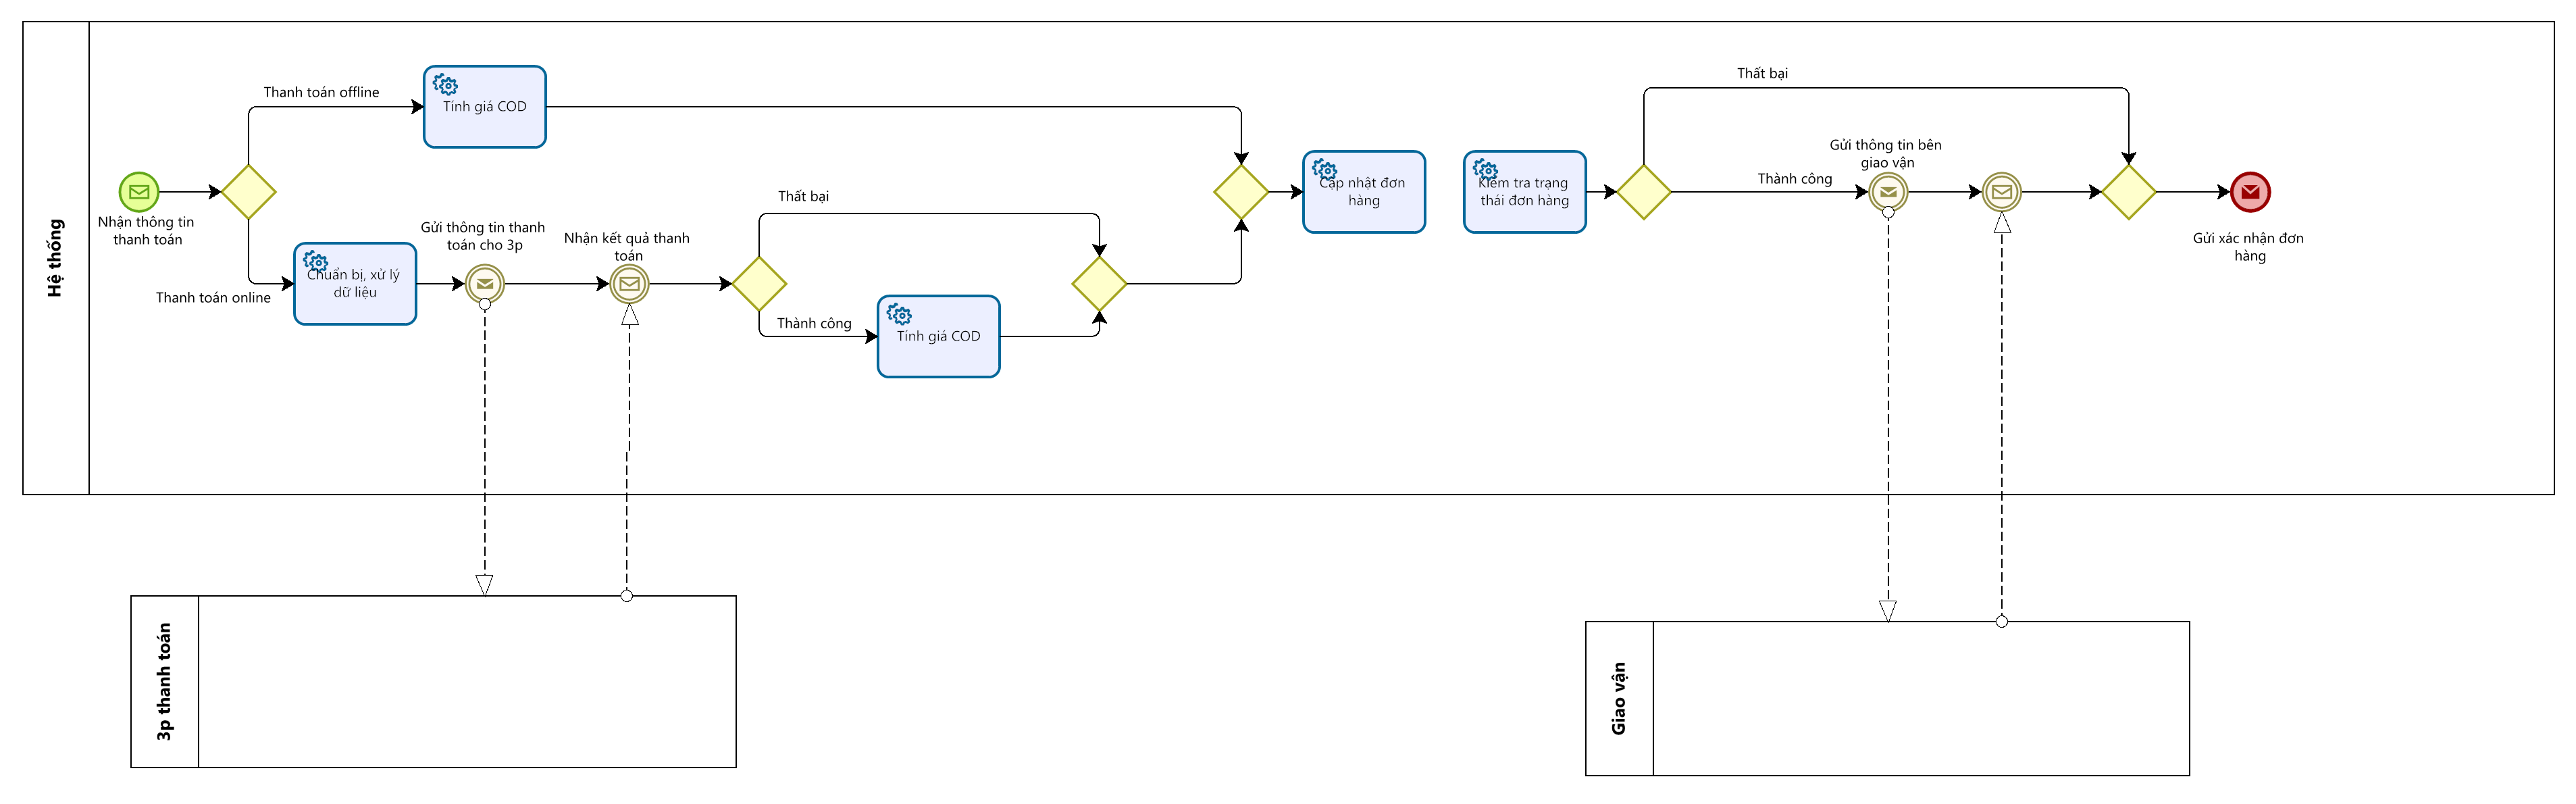
\includegraphics[width=9cm]{img/BPMN/customer_buy/customer_payment.png}
	\newline
	\caption{Lược đồ BPMN cho quy trình tạo đơn hàng}
\end{figure}

Đây là một quy trình con chứa quy trình tạo đơn hàng. Quy trình bắt đầu từ sự kiện nhận thông tin đơn hàng, hệ thống thực hiện kiểm tra đơn hàng có cần thực hiện chuyển kho không, nếu có sẽ tiến hành chuyển. Sau cùng hệ thống sẽ cập nhật thông tin đơn hàng.


\subsection{Quản lý sự kiện}

\subsubsection{Thêm sự kiện}

\begin{figure}[!htp]
	\centering
	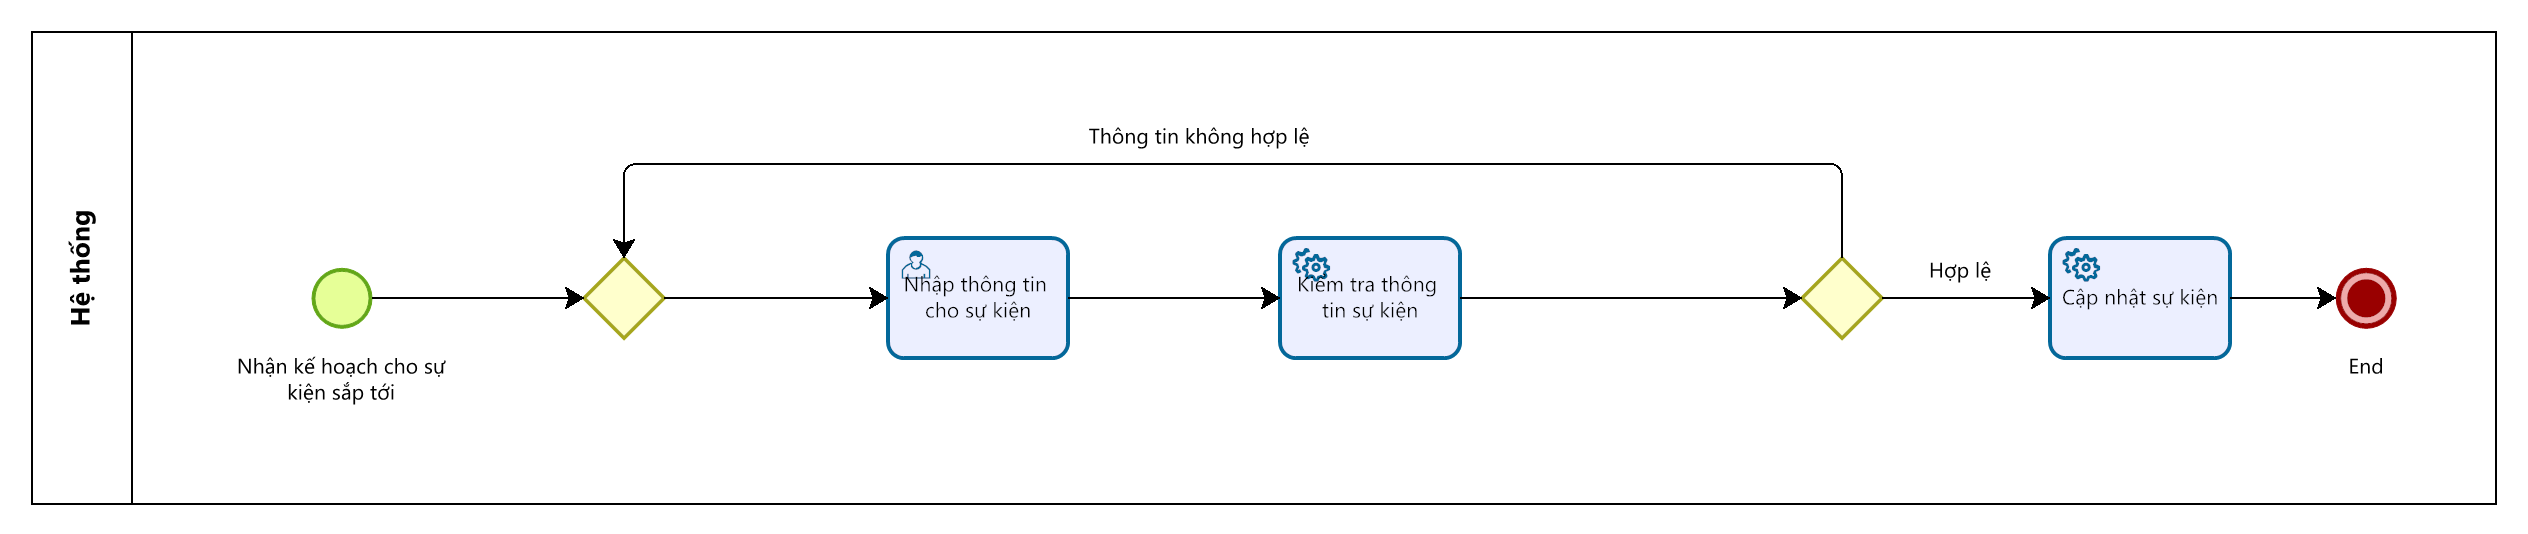
\includegraphics[width=14cm]{img/BPMN/event/add_event.png}
	\newline
	\caption{Lược đồ BPMN cho quy trình thêm sự kiện}
\end{figure}

Quy trình được bắt đầu bởi sự kiện nhận thông tin cho sự kiện sắp tới, sau khi nhận được thông tin sự kiện mới thì quản trị viên nhập thông tin cho sự kiện và xác nhận tạo sự kiện. Sau khi thông tin sự kiện mới được gửi đi thì hệ thống sẽ kiểm tra thông tin sự kiện có hợp lệ hay không, nếu hợp lệ thì cập nhật sự kiện mới vào hệ thống và kết thúc quy trình, nếu không hợp lệ thì quản trị viên cần quay lại task nhập lại thông tin cho sự kiện.

\subsubsection{Sửa sự kiện}

\begin{figure}[!htp]
	\centering
	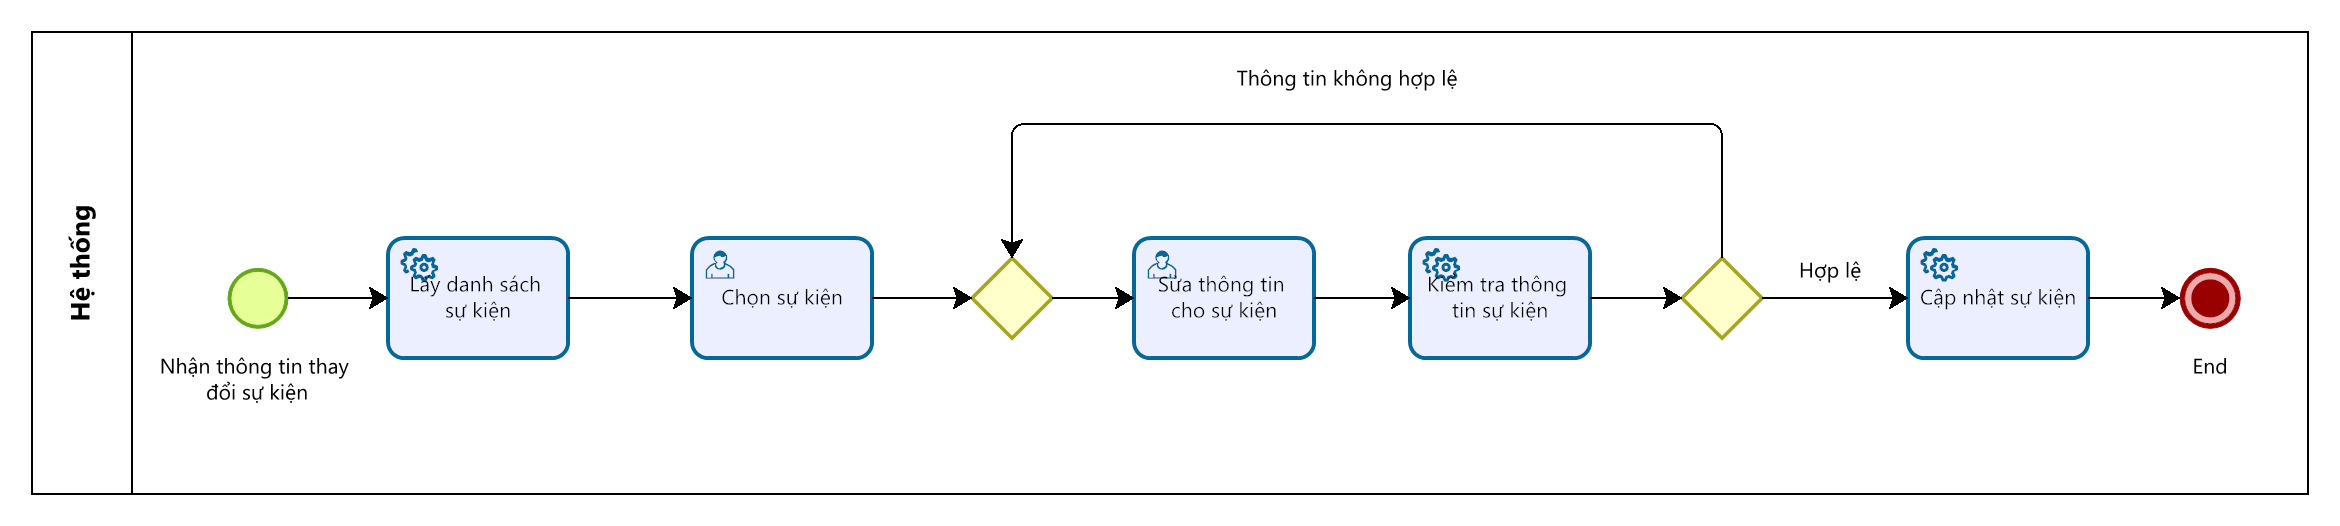
\includegraphics[width=14cm]{img/BPMN/event/edit_event.png}
	\newline
	\caption{Lược đồ BPMN cho quy trình chỉnh sửa sự kiện}
\end{figure}

Quy trình được bắt đầu bởi sự kiện nhận thông tin thay đổi sự kiện, sau khi nhận được thông tin sự kiện cần cập nhật thì quản trị viên chọn sự cần cần sửa, sau đó nhập thông tin cho sự kiện và xác nhận cập nhật sự kiện. Sau khi thông tin cập nhật sự kiện được gửi đi thì hệ thống sẽ kiểm tra thông tin sự kiện có hợp lệ hay không, nếu hợp lệ thì cập nhật lại sự kiện vào hệ thống và kết thúc quy trình, nếu không hợp lệ thì quản trị viên cần quay lại task nhập lại thông tin cho sự kiện.
\newpage
\subsubsection{Xóa sự kiện}

\begin{figure}[!htp]
	\centering
	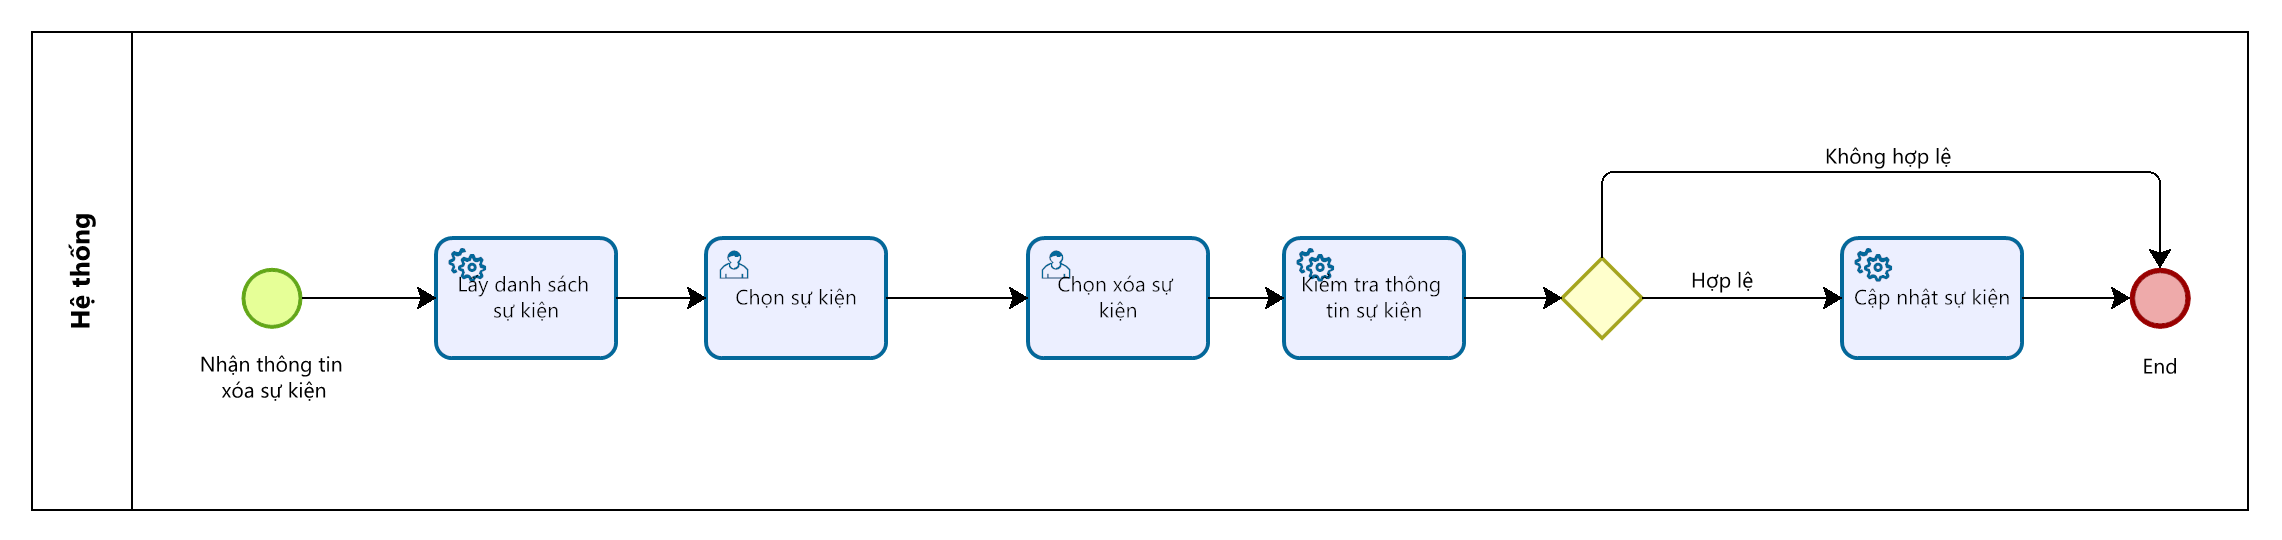
\includegraphics[width=14cm]{img/BPMN/event/delete_event.png}
	\newline
	\caption{Lược đồ BPMN cho quy trình xóa sự kiện}
\end{figure}

Quy trình được bắt đầu bởi sự kiện nhận thông tin xóa sự kiện, sau khi nhận được thông tin sự kiện cần cập nhật thì quản trị viên chọn sự cần cần xóa và chọn xóa sự kiện. Sau khi thông tin sự kiện cần xóa được gửi đi thì hệ thống sẽ kiểm tra thông tin sự kiện có hợp lệ hay không, nếu hợp lệ thì cập nhật xóa sự kiện khỏi hệ thống và kết thúc quy trình, nếu không hợp lệ thì thông báo thất bại và kết thúc quy trình.


\subsection{Khách hàng mua hàng trực tiếp}
\begin{figure}[!htp]
	\centering
	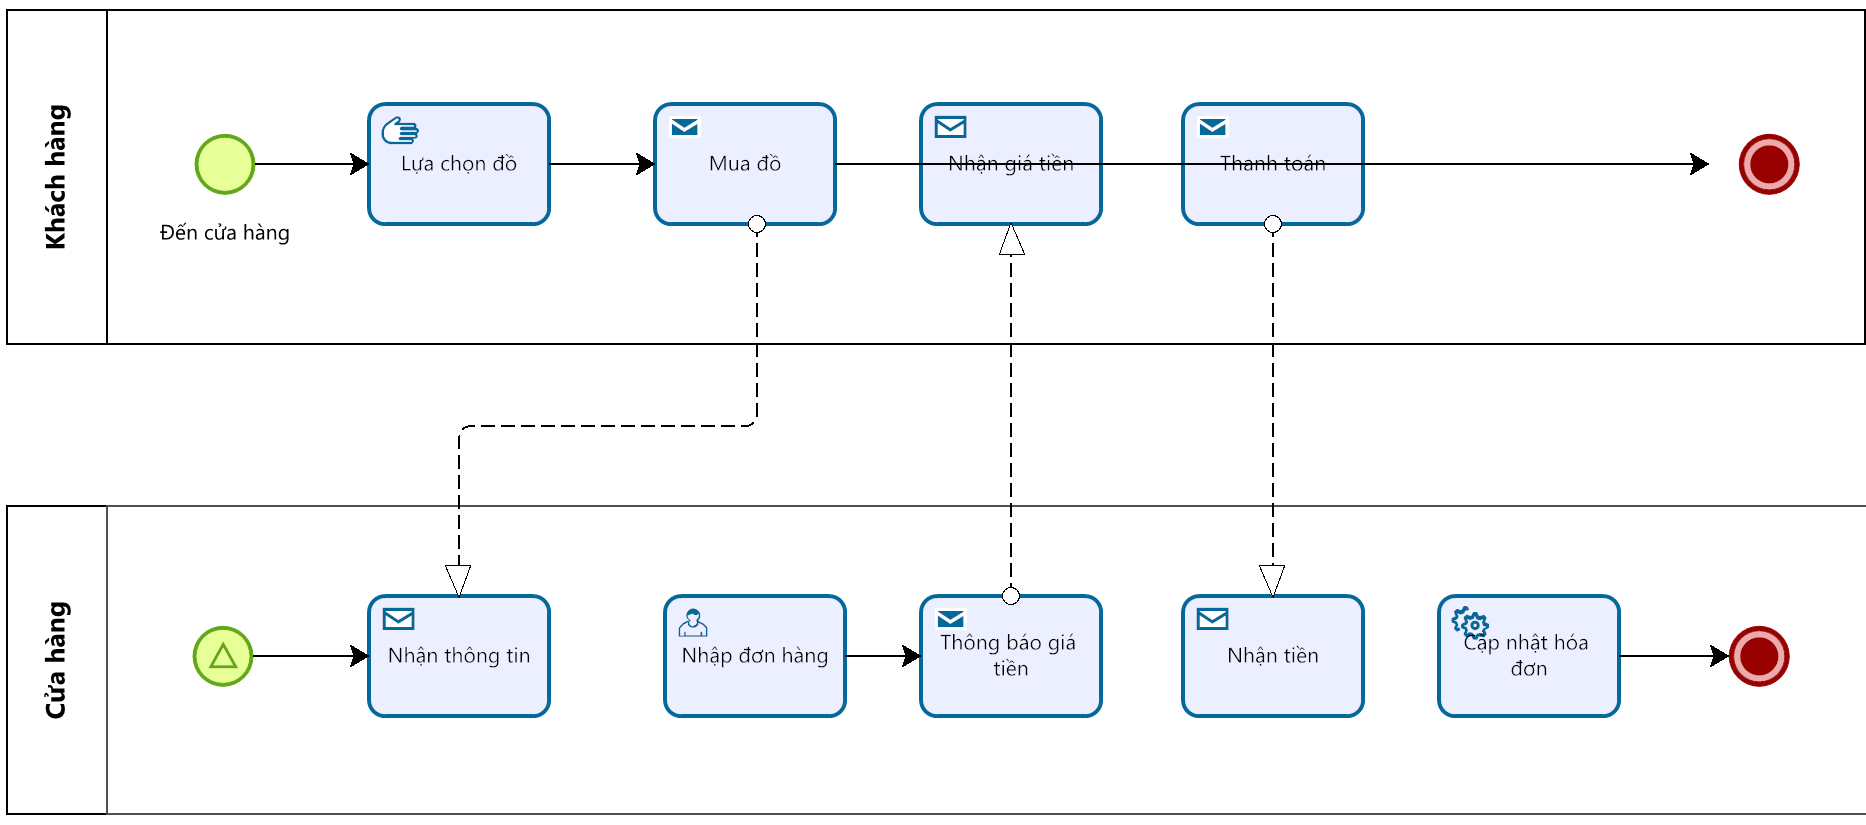
\includegraphics[width=13cm]{img/BPMN/Hien/Customer_buyOffline.png}
	\newline
	\caption{Lược đồ BPMN cho quy trình khách hàng mua hàng trực tiếp}
\end{figure}

Khách hàng sau khi đến cửa hàng sẽ thực hiện chọn sản phẩm và thông báo cho nhân viên sản phẩm của mình. Nhân viên thực hiện nhập đơn hàng và báo giá cho khách hàng. Khách hàng nhận thông tin và thực hiện thanh toán. Nhân viên nhân tiền và cập nhật hóa đơn trên hệ thống

\newpage

\subsection{Đăng nhập}
\begin{figure}[!htp]
	\centering
	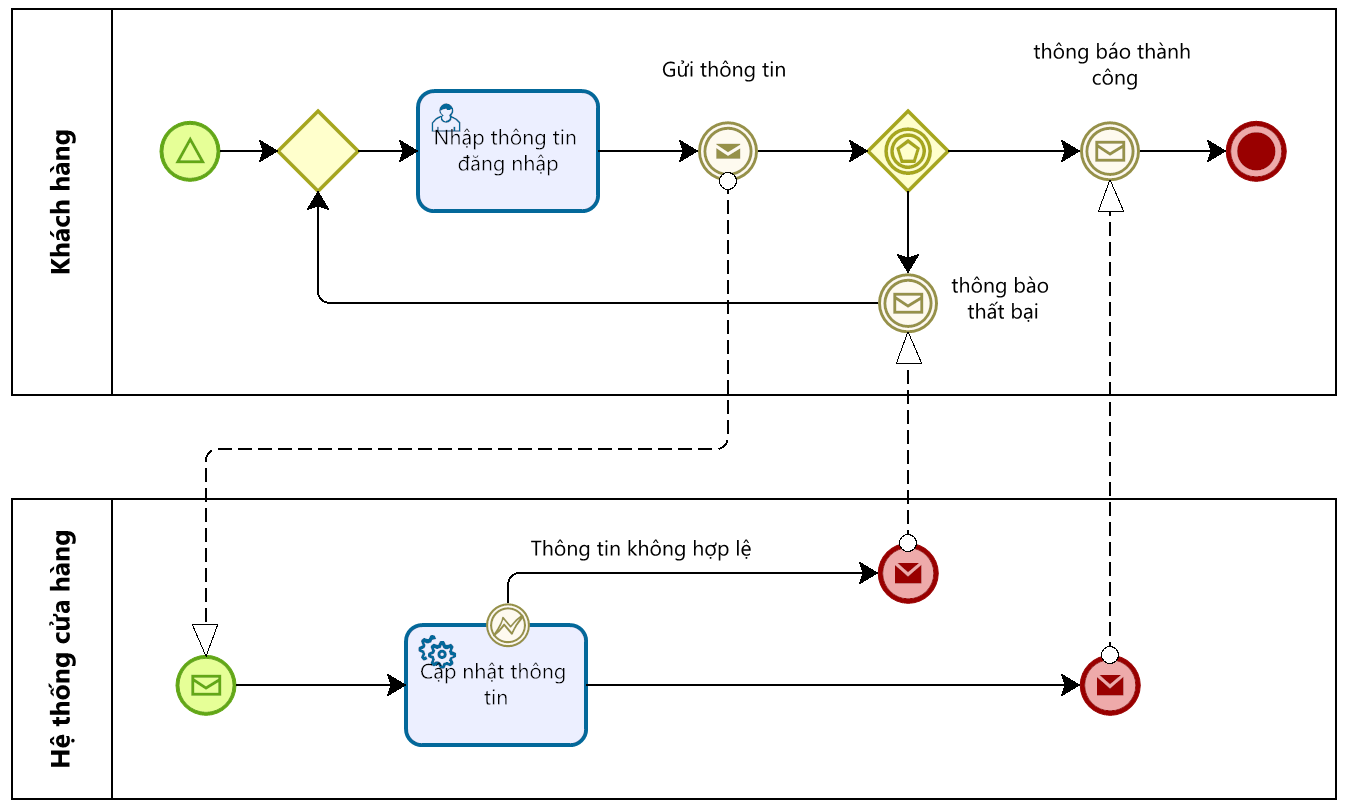
\includegraphics[width=10cm]{img/BPMN/Hien/Customer_login.png}
	\newline
	\caption{Lược đồ BPMN cho quy trình đăng nhập}
\end{figure}

Người dùng truy cập hệ thống nhập thông tin đăng nhập và chọn đăng nhập. Hệ thống thực hiện kiểm tra thông tin và trả thông báo thành công hoặc thất bại. Nếu thất bại sẽ yêu cầu người dùng đăng nhập lại

\subsection{Đăng ký tài khoản}
\begin{figure}[!htp]
	\centering
	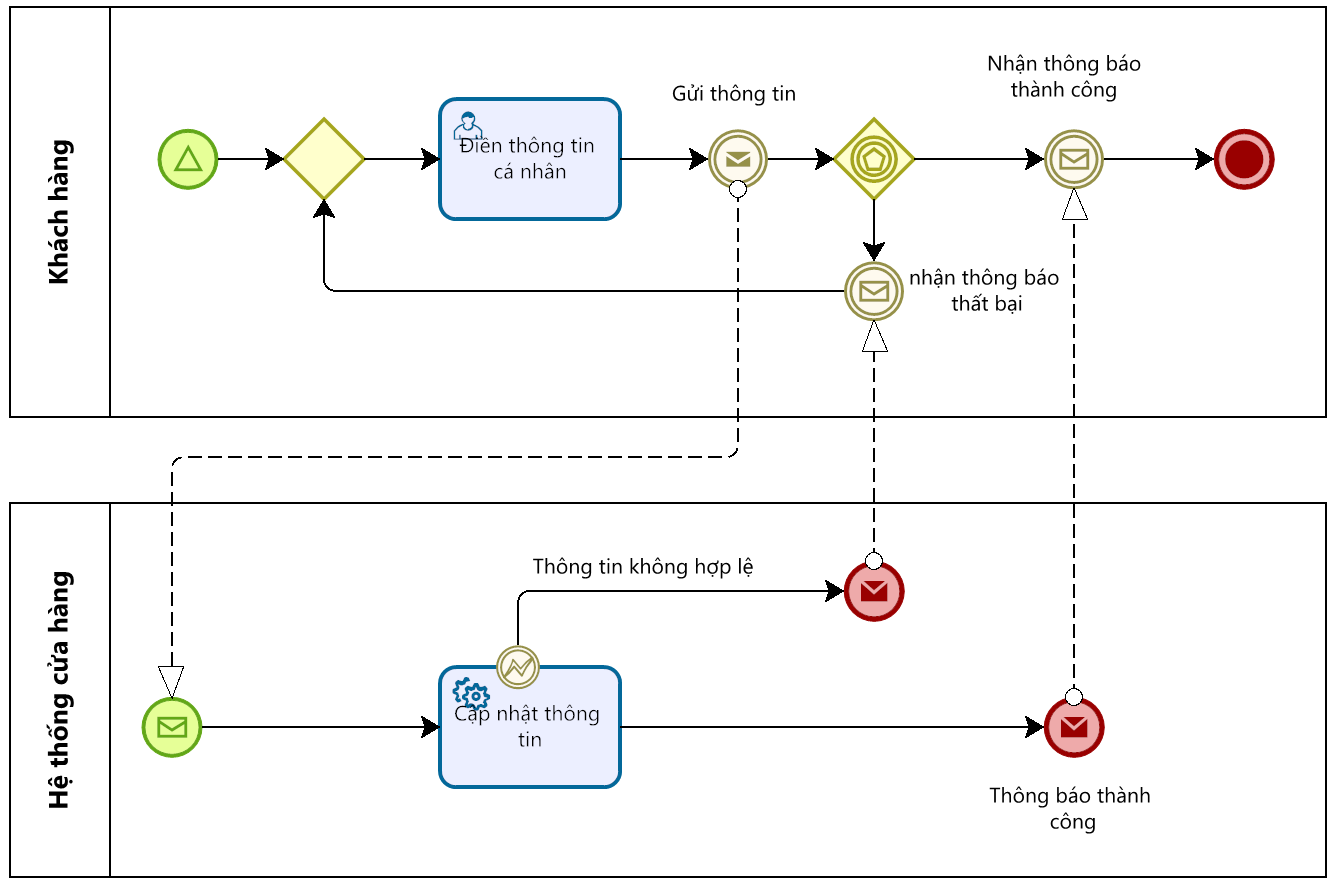
\includegraphics[width=10cm]{img/BPMN/Hien/Customer_register.png}
	\newline
	\caption{Lược đồ BPMN cho quy trình đăng ký tài khoản mới}
\end{figure}

Người dùng nhập thông tin cá nhân và chọn đăng ký. Hệ thống nhận thông tin và cập nhật. Hệ thống thông báo thành công nếu thành công và thông báo thất bại nếu thông tin không hợp lệ


\subsection{Làm mới mật khẩu}
\begin{figure}[!htp]
	\centering
	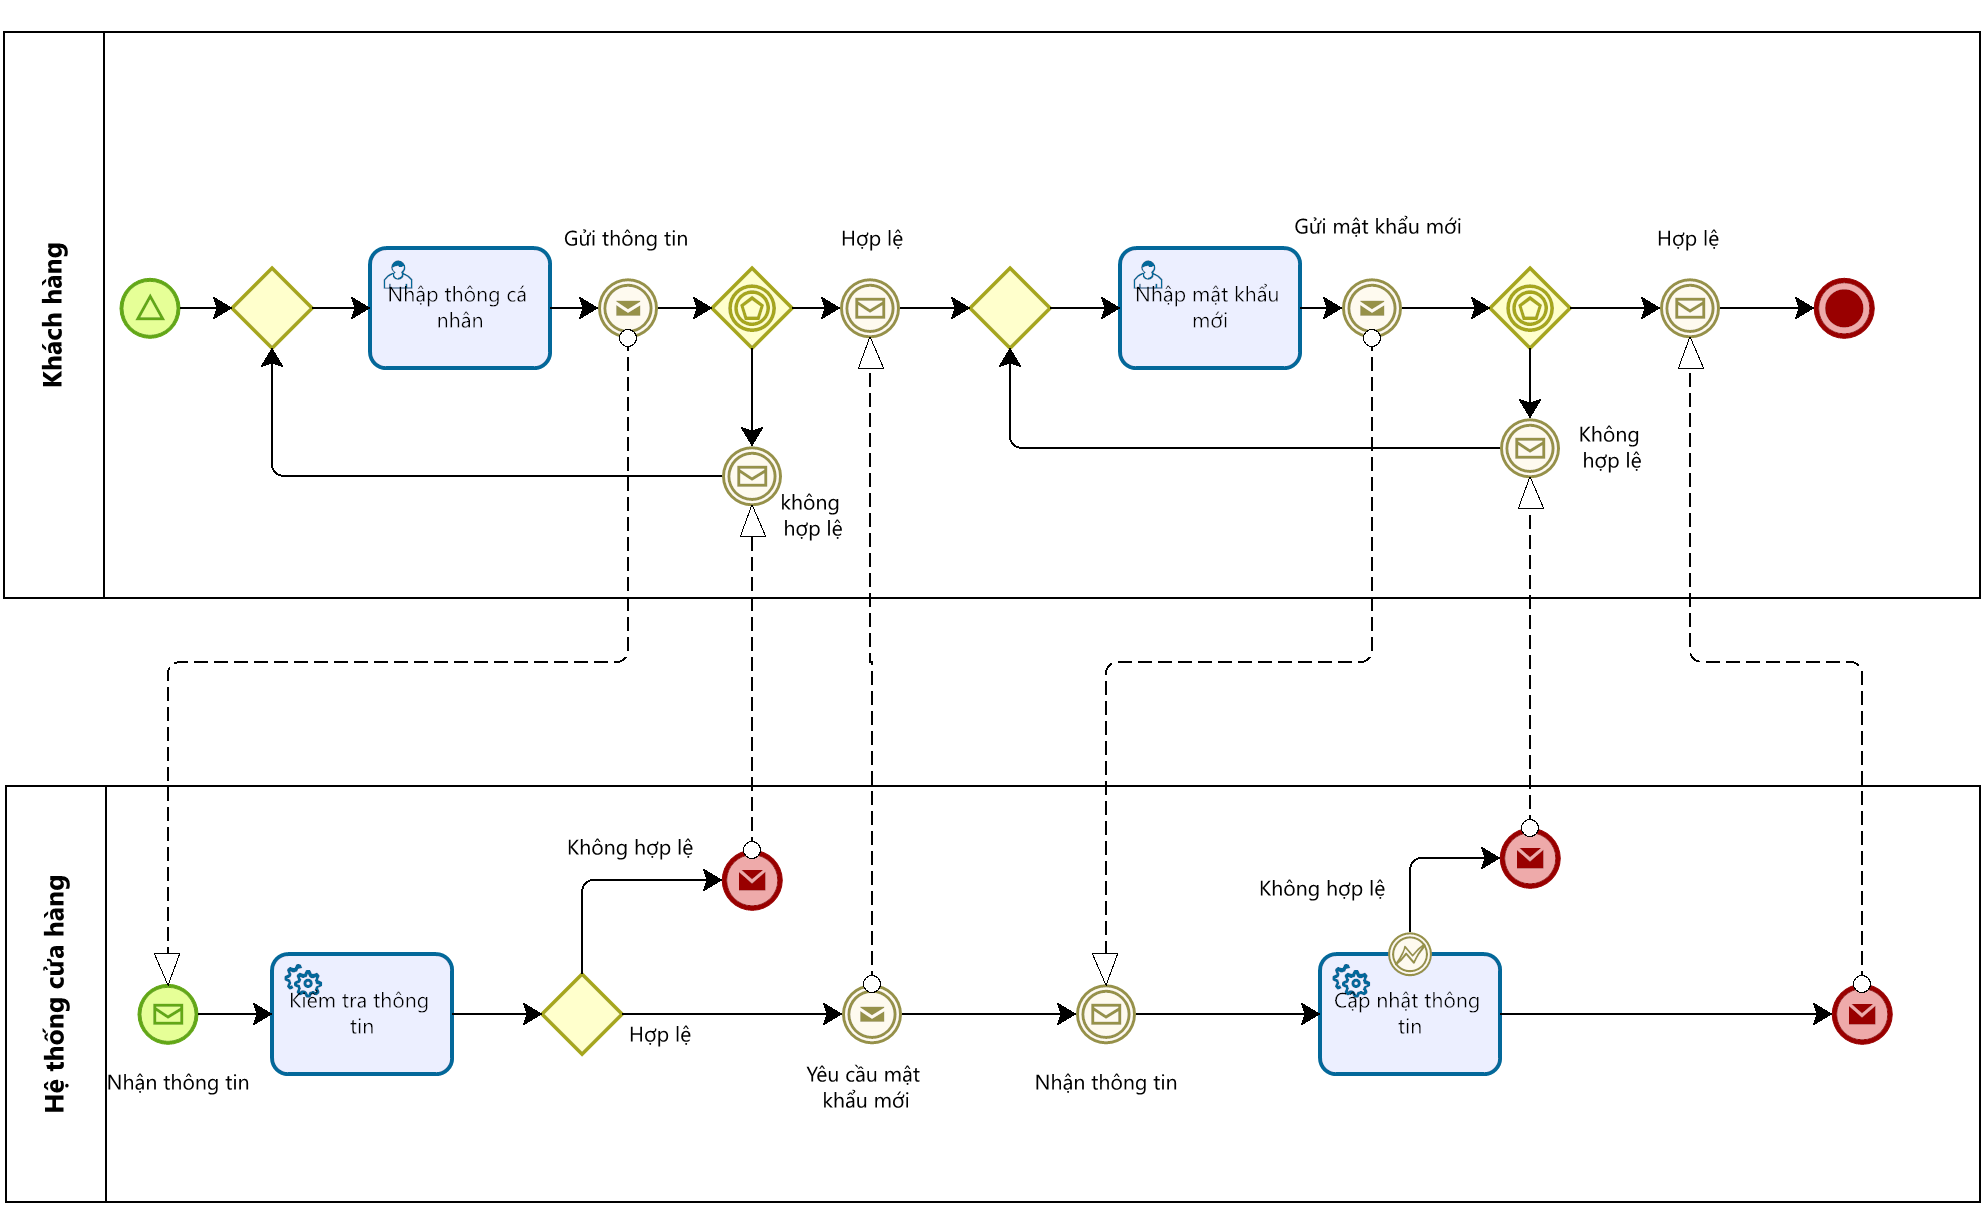
\includegraphics[width=14cm]{img/BPMN/Hien/Customer_resetPassword.png}
	\newline
	\caption{Lược đồ BPMN cho quy trình làm mới mật khẩu}
\end{figure}

Người dùng nhập thông tin cá nhân và gửi. Hệ thống kiểm tra thông tin, nếu hợp lệ sẽ yêu cầu mật khẩu mới từ người dùng; ngược lại sẽ yêu cầu người dùng nhập lại thông tin. Sau khi người dùng nhập mật khẩu mới và gửi, hệ thống sẽ cập nhật thông tin và gửi thông báo thành công, nếu mật khẩu không hợp lệ sẽ yêu cầu người dùng nhập lại.
\newpage

\subsection{Quản lý chi nhánh}
\begin{figure}[!htp]
	\centering
	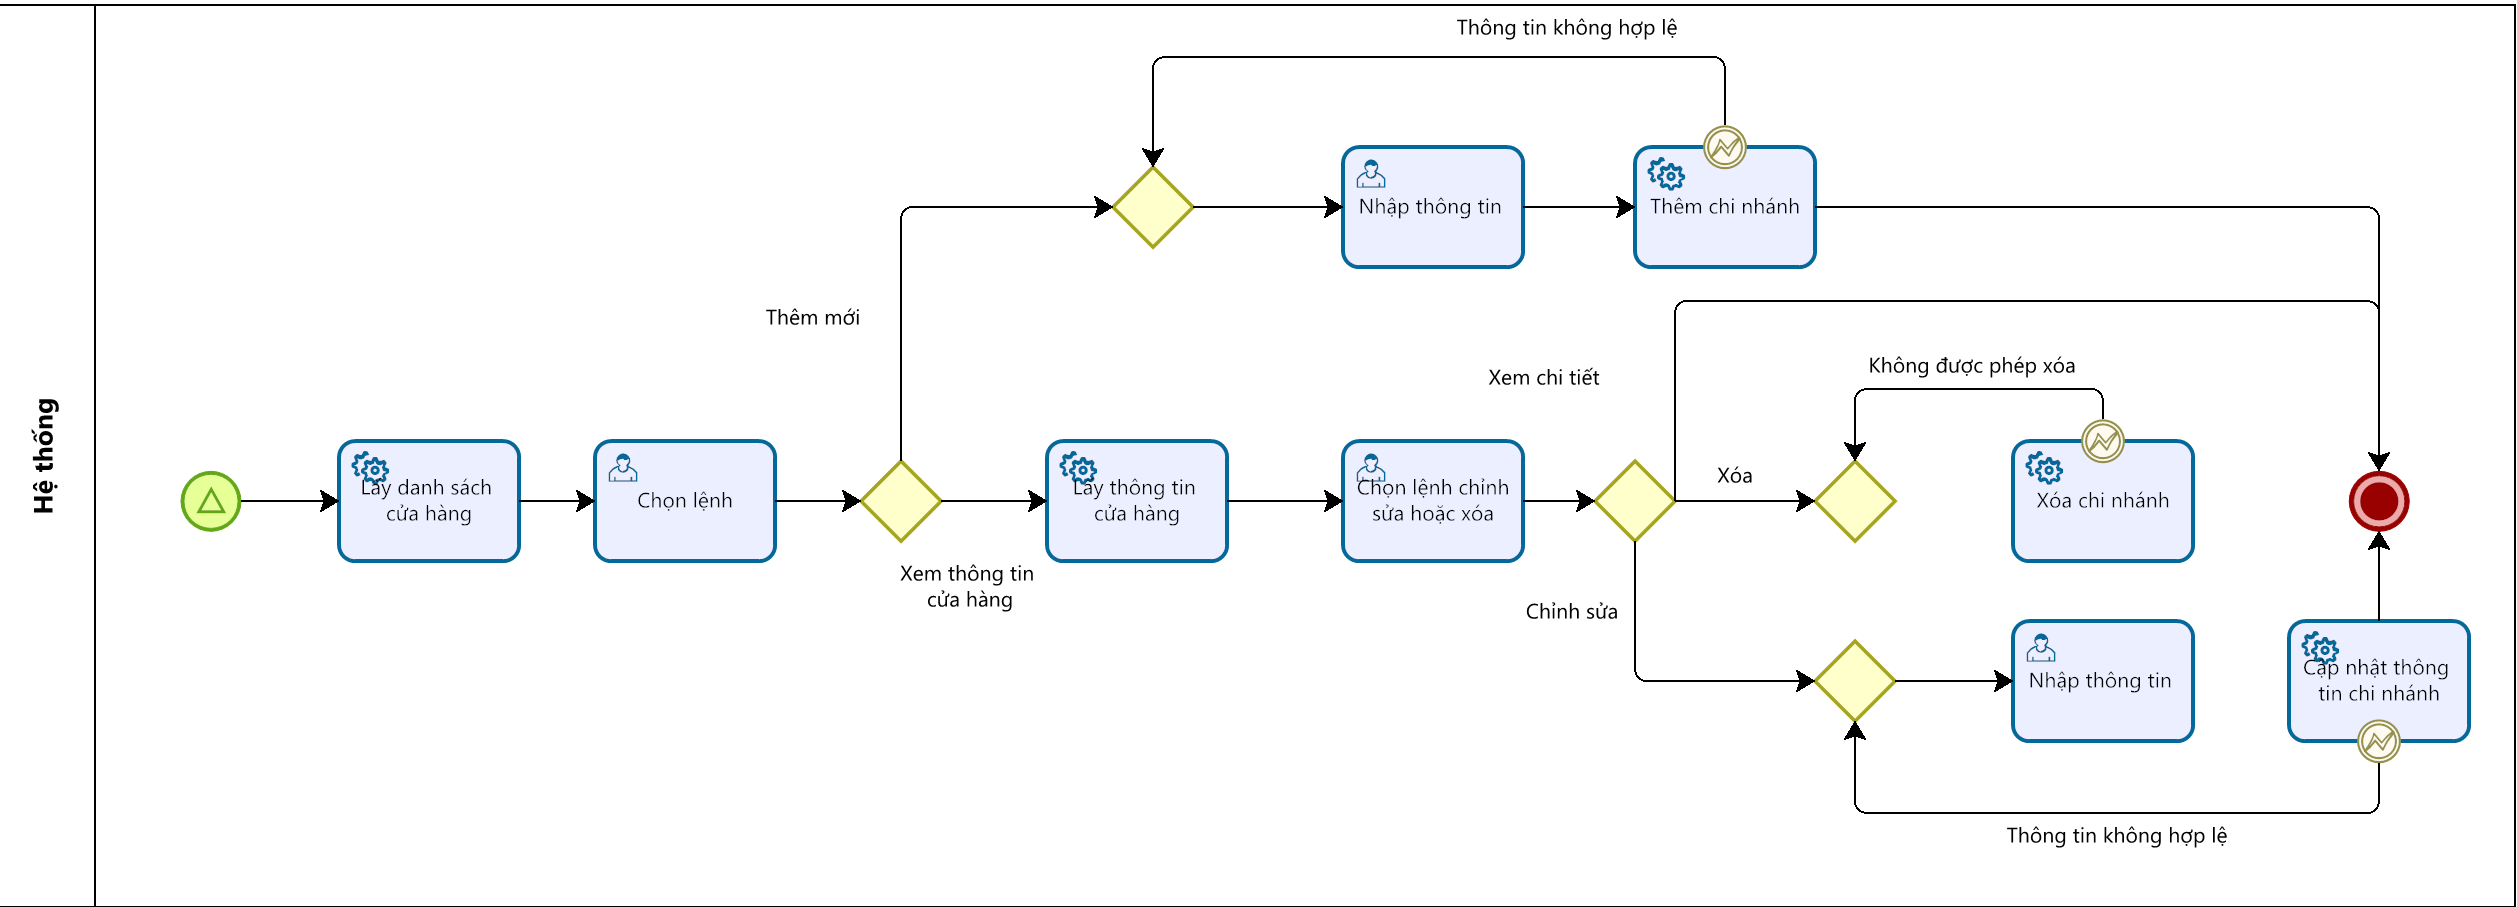
\includegraphics[width=16cm]{img/BPMN/Hien/Branch_management.png}
	\newline
	\caption{Lược đồ BPMN cho quy trình quản lý chi nhánh}
\end{figure}

Khi quản trị viên truy cập, hệ thống sẽ lấy danh sách chi nhánh. Quản trị viên thực hiện thêm mới hoặc xem thông tin chi nhánh. Nêu thêm mới, quản trị viên sẽ nhập thông tin chi nhánh mới và cập nhật hệ thống. Nâu có thông tin không hợp lệ, hệ thống sẽ yêu cầu nhập lại thông tin. Nếu xem thông chi nhánh, hệ thống sẽ lấy thông tin chi tiết của chi nhánh đó. Quản trị viên có thể chỉ xem thông tin chi nhánh, chỉnh sửa thông tin hoặc xóa chi nhánh. Nếu chọn xóa, hệ thống sẽ kiểm tra và xóa nếu hợp lệ, ngược lại sẽ hiện thông tin chi tiết chi nhánh. Nếu chọn chỉnh sửa, hệ thống yêu cầu nhập thông tin sẽ kiểm tra thông tin nếu hợp lệ sẽ cập nhật thông tin, ngược lại sẽ yêu cầu nhập lại thông tin


\subsection{Quản lý nhân viên}
\begin{figure}[!htp]
	\centering
	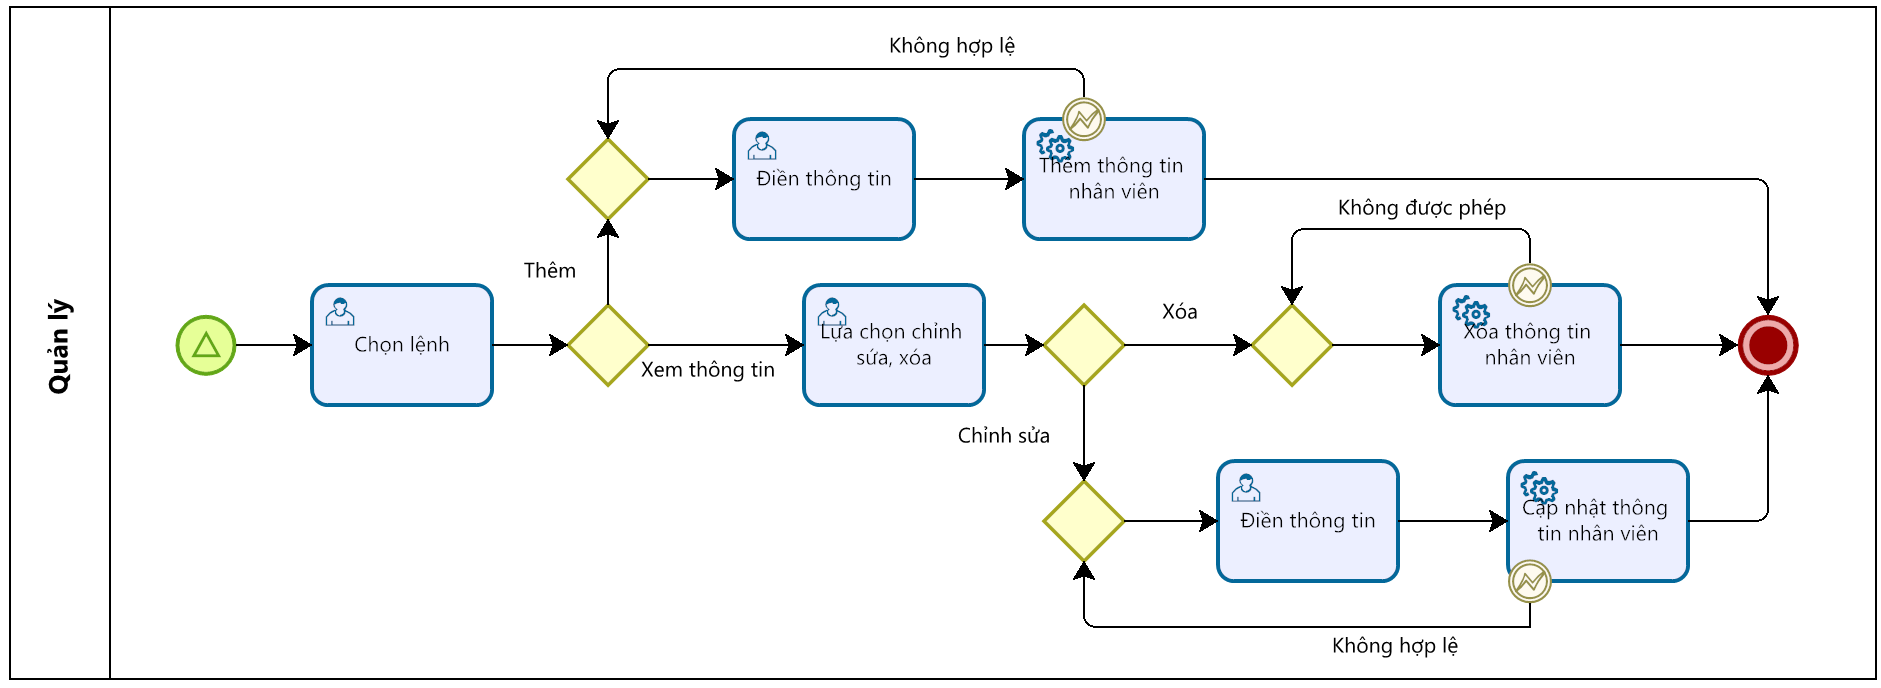
\includegraphics[width=16cm]{img/BPMN/Hien/Employee_Management.png}
	\newline
	\caption{Lược đồ BPMN cho quy trình quản lý nhân viên}
\end{figure}

Khi quản trị viên truy cập, hệ thống sẽ lấy danh sách nhân viên. Quản trị viên thực hiện thêm mới hoặc xem thông tin nhân viên. Nêu thêm mới, quản trị viên sẽ nhập thông tin nhân viên mới và cập nhật hệ thống, nếu có thông tin không hợp lệ, hệ thống sẽ yêu cầu nhập lại thông tin. Nếu xem thông nhân viên, hệ thống sẽ lấy thông tin chi tiết của nhân viên đó. Quản trị viên có thể chỉ xem thông tin nhân viên, chỉnh sửa thông tin hoặc xóa nhân viên. Nếu chọn xóa, hệ thống sẽ kiểm tra và xóa nếu hợp lệ, ngược lại sẽ hiện thông tin chi tiết nhân viên. Nếu chọn chỉnh sửa, hệ thống yêu cầu nhập thông tin sẽ kiểm tra thông tin nếu hợp lệ sẽ cập nhật thông tin, ngược lại sẽ yêu cầu nhập lại thông tin

\subsubsection*{Tạo yêu cầu thêm, xóa nhân viên}
\begin{figure}[!htp]
	\centering
	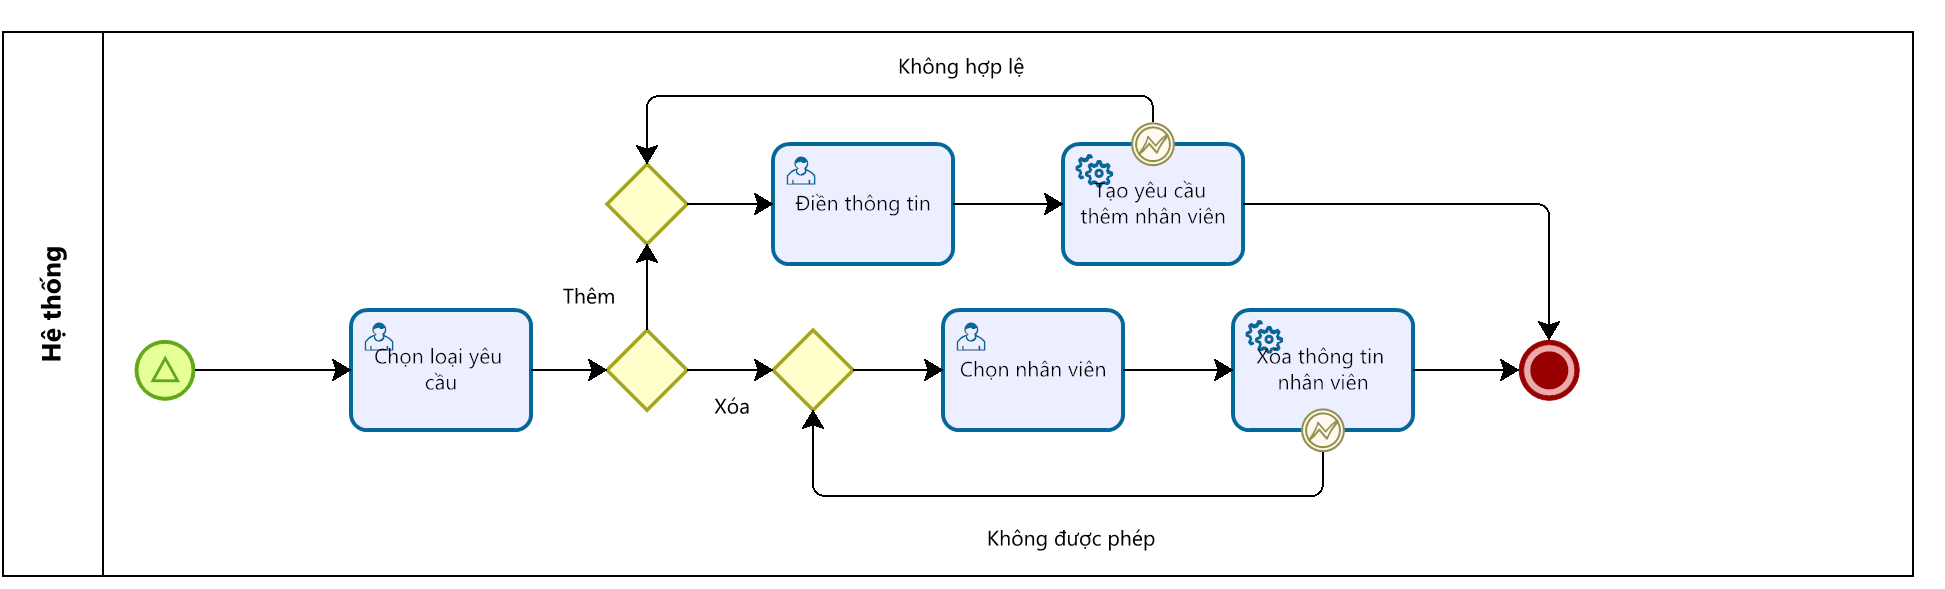
\includegraphics[width=14cm]{img/BPMN/Hien/Employee_request.png}
	\newline
	\caption{Lược đồ BPMN cho quy trình tạo yêu cầu thêm, xóa nhân viên}
\end{figure}

Khi truy cập hệ thống, quản lý có thể chọn loại yêu cầu. Nếu là yêu cầu thêm, hệ thống yêu cầu nhập thông tin nhân viên mới và tạo yêu cầu, nếu thông tin không hợp lệ sẽ phải nhập lại thông tin. Nếu là yêu cầu xóa, hệ thống yêu cầu chọn nhân viên và tạo yêu cầu, nếu không hợp lệ sẽ yêu cầu chọn nhân viên khác